\section{Effect of Problem Domain Size and Precision} \label{sec:res-size}

\subsection{Change in X and Y Domain Size}

\begin{figure}
	% dat=pd.concat([large, medium, small])
% dat["rel"]=u.relmingroup(dat,by=u.col.size+u.col.stencil)
% fastest=u.groupmin(dat, by=u.col.problem+u.col.variant+u.col.storage)
	% u.barplot(fastest[fastest["unstructured"]&(fastest["size-z"]==64)&(fastest["stencil"]=="laplap")], cat=u.col.size, grp=u.col.variant, y="rel", tickrot=0)
	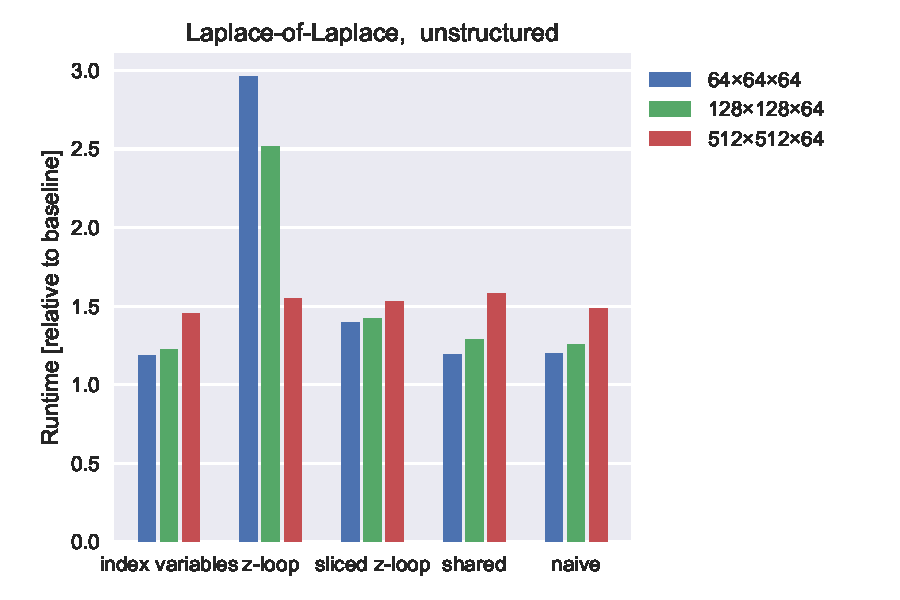
\includegraphics[scale=0.75]{variants-gridsizes.pdf}
	\caption{\label{fig:variants-gridsizes} Relative runtime of different variants of the Laplace-of-Laplace benchmark at different X-Y-sizes with respect to the fastest regular variant. For each bar, the fastest storage variant is considered (fastest of compression/chasing/z-curves).}
\end{figure}

We have evaluated combinations of grid storage and access variants for the three stencils on grids of X-Y size $64\times 64$ (small grid), $128\times 128$ (medium grid) and $512\times 512$ (large grid). Naturally, larger problem sizes lead to longer run times in all variants. More intrestingly however, increases in the X-Y-domain size affect the unstructured variants more negatively than the regular ones.

For small domains, the runtimes of unstructured variants are generally close to those of their regular counterparts. With increased domain size, there is an increase in the relative slowdown of the unstructured variant with respect to the fastest regular implementation. We assume this is due to cache sizes; while in smaller grids, entire neighborship tables and cell values remain cached, larger grids necessitate larger neighborship tables which cannot fit into the cache together with the cell values as a whole. Figure \ref{fig:variants-gridsizes} shows this trend for the Laplace-of-Laplace benchmark, but the same characteristics apply to the other stencils as well.

The \emph{z-loop} grid access variant is the only exception to the described charateristics. Its relative slowdown decreases for larger grid sizes. This is probably due to two reasons. First, the z-loop variants already suffer from low occupancy in large grids. In small grids, occupancy is even lower, not making use of the complete parallelism capabilities of the GPU. Second, in small grids, the neighborship table may be in cache in its entirety after one read. This allows subsequent neighborship table accesses to be practically free. This offsets the supposed optimization of the z-loop variant, which aims to reduce the number of reads of neighborship table entries. This optimization only begins to provide a benefit in large grids.

\subsection{Change in Z domain size}

\begin{figure}
	% dat = pd.read_csv("results/ultimate-reformat.csv")
	% dat["rel"] = u.relmingroup(dat, by=u.col.stencil+u.col.size)
	% u.lineplot(dat[(dat["stencil"]=="laplap")&(dat["variant"]=="idxvar")&dat["z-curves"]], x="size-z", y="rel")
% fig=u.plotdone(legend=0)
	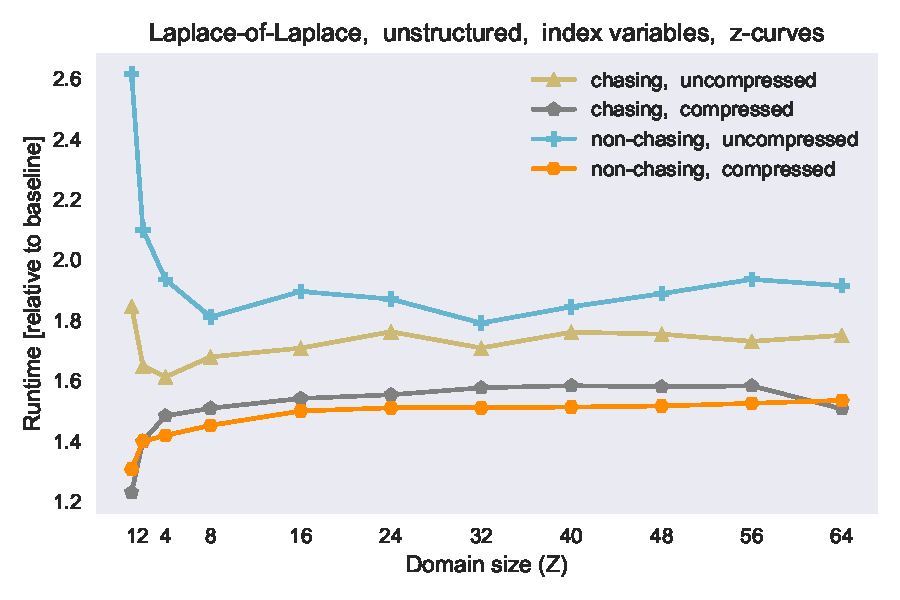
\includegraphics[scale=0.75]{laplap-idxvar-z-sizes.pdf}
	\caption{\label{fig:laplap-z-sizes} Relative slowdowns of the Laplace-of-Laplace stencil on unstructured grids of various Z-sizes. Baseline: fastest regular grid implementation.}
\end{figure}

Considering the relative slowdowns of unstructured grid implementations across different sizes in the Z-dimension reveals some interesting patterns. Given a $512\times 512$ base grid with various Z-sizes ranging from $1$ to $64$, we analyzed the overhead of switching to unstructured grids using various storage and access methods.

Figure \ref{fig:laplap-z-sizes} plots the relative slowdowns as a function of the Z-size for the Laplace-of-Laplace stencil using the index variables access method. The plot is representative of all other stencils and access methods. We make the following two observations:

For uncompressed storage, the overhead generally decreases with increasing domain size in the Z-dimension. This can be most clearly be seen in grids with no pointer chasing. This trend can be explained by the regularity of the grid in the Z-dimension, which some of the optimized implementations make use of. Theoretically, only one lookup to determine neighboring indices is required for all cells in a grid with equal X- and Y-coordinates. Optimized grid access variants make use of this fact to reduce the number of neighborship table reads. Even the unoptimized variants profit from the Z-regularity, as neighborship information appears to be mostly kept in the caches.


\subsection{Effect of Floating Point Precision}

We observed no significant differences in the relative slowdown when using single-precision floating point data types instead of double-precision data types. As expected, the absolute runtimes decrease with lower precision. This happens in the same proportions for both regular grid and unstructured grid implementations -- both are roughly $40\%$ faster than double-precision speeds.

As it appears to have no effect on the characteristics of our benchmarks, we consistently used double precision data types in all other experiments apart from this section.

\begin{verbatim}
% TODO
% - effect of Z-size increase
%   -> graph per variant (choose best-looking storage strategy if all similar)
%   -> reiterate how this shows that z regularity is made use of in certain variants
%   -> point to latency for first neighbor lookups that cannot be hidden
% - effect of XY-size change
%   -> smaller sizes 128x128x64
%   -> larger sizes 512x512x64
% - effect of precision
%   -> grouped bar graph double vs single; keep short
\end{verbatim}